\documentclass{beamer}
\usetheme{metropolis}
\metroset{sectionpage=none}
\definecolor{TUGreen}{rgb}{0.517,0.721,0.094}
\setbeamercolor{background canvas}{bg=white,fg=black}
\setbeamercolor{frametitle}{bg=white,fg=TUGreen}
\setbeamercolor{alerted text}{fg=TUGreen}
\setbeamerfont{bibliography item}{size=\tiny}
\setbeamerfont{bibliography entry author}{size=\tiny}
\setbeamerfont{bibliography entry title}{size=\tiny}
\setbeamerfont{bibliography entry location}{size=\tiny}
\setbeamerfont{bibliography entry note}{size=\tiny}


\usepackage[T1]{fontenc}
\usepackage[utf8]{inputenc}
\usepackage[english,german,ngerman]{babel}
\usepackage{tikz}
\usepackage{pgfplots}
\usepackage{booktabs}
\usepackage{tabularx}
\pgfplotsset{compat=1.16}
\usepgfplotslibrary{groupplots}
\usepackage{grffile}
\usepackage{caption}
\captionsetup[figure]{font=tiny,labelfont=tiny}
\renewcommand{\figurename}{Abb.}
\usepackage{subcaption}
\makeatletter
\newcommand*{\currentname}{\@currentlabelname}
\setbeamertemplate{footline}[frame number]{}
\setbeamertemplate{frametitle}{%
	\nointerlineskip%
	\begin{beamercolorbox}[%
		wd=\paperwidth,%
		sep=0pt,%
		leftskip=\metropolis@frametitle@padding,%
		rightskip=\metropolis@frametitle@padding,%
		]{frametitle}%
		\begin{minipage}[t]{42ex}
			\metropolis@frametitlestrut@start%
			\insertframetitle%
			\nolinebreak%
			\metropolis@frametitlestrut@end%
		\end{minipage}
		\hfill
		\begin{minipage}[t]{14ex}
			\vspace{-1.6ex}
			
\includegraphics[height=2.2ex,keepaspectratio]{tud_logo_rgb}
		\end{minipage}
	\end{beamercolorbox}%
}
\makeatother

\title{Segmentierung der Marsoberfläche mit Hilfe von unüberwachtem tiefen Clustering}
\subtitle{Bachelorarbeit Abschlusspräsentation}
\author{Merlin Scholz}
\date{\today}
\institute[TU Dortmund]{Mustererkennung,\\ Informatik XII, Technische Universität Dortmund}

\begin{document}
\maketitle

\begin{frame}{Inhalt}
\tableofcontents
\end{frame}


\section{Motivation}
\begin{frame}{Motivation: Neuronale Netze zur Bildsegmentierung}
\begin{itemize}
	\item Neuronale Netzwerke werden oft zur Bildsegmentierung genutzt
	\item Gewöhnlich als Voraussetzung: Vorhandene Ground Truth
\end{itemize}% TODO Bild
\end{frame}

\begin{frame}{Motivation: (Fehlende) Ground Truths}
	\begin{minipage}{0.68\textwidth}
\begin{itemize}
	\item Ground Truths sind nicht immer vorhanden
	\item Beispiel: Marsoberfläche
	\begin{itemize}
		\item Zu großer Datensatz
		\item Notwendigkeit von Domänenexperten
	\end{itemize}
	\item Lösungsansatz:
	\begin{itemize}
		\item Anfangs zufällige Klassifizierung durch Segmentierungsalgorithmus weiter optimieren
	\end{itemize}
\end{itemize}

\end{minipage}
\hfill
\begin{minipage}{0.2\textwidth}
	\begin{figure}[h!]
		\begin{subfigure}{\textwidth}
			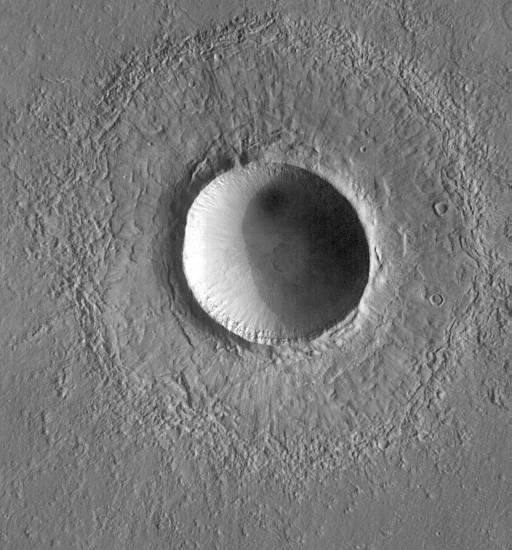
\includegraphics[width=\textwidth,keepaspectratio]{gfx/Gre13_01.jpg}
		\end{subfigure}
		\begin{subfigure}{\textwidth}
			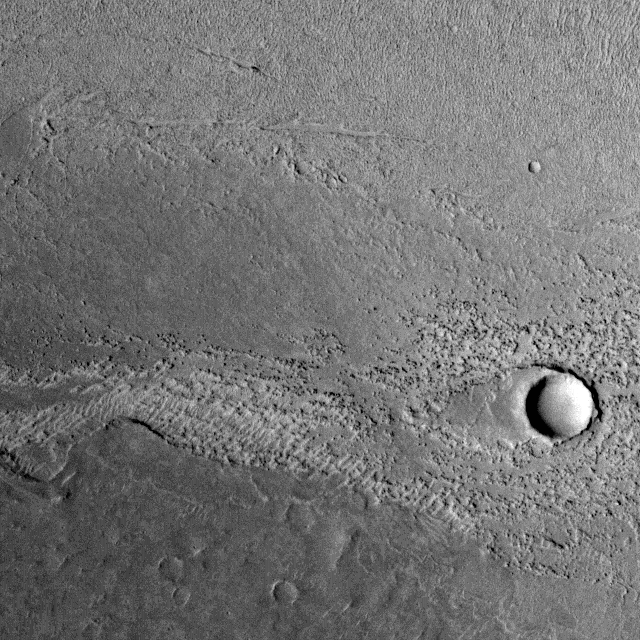
\includegraphics[width=\textwidth,keepaspectratio]{gfx/p03_02.png}
		\end{subfigure}
		\begin{subfigure}{\textwidth}
			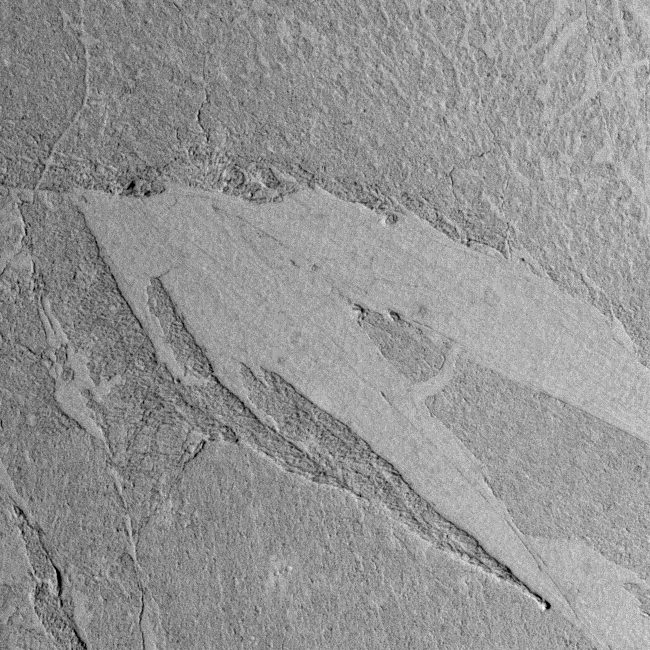
\includegraphics[width=\textwidth,keepaspectratio]{gfx/p03_03.png}
		\end{subfigure}
		\caption{Beispielaufnahmen, teilweise aus \cite{greeley_13}}
	\end{figure}
\end{minipage}
\end{frame}

%\section{Grundlagen}

\section{Verwandte Arbeiten}



\begin{frame}[allowframebreaks]{Verwandte Arbeiten: Unsupervised Deep Embedding for Clustering Analysis \cite{junyuan_16}}
\begin{itemize}
	\item Unüberwachtes Lernen der Segmentierung in $k$ Segmente
	\item Geschieht durch Zuteilen von Punkten in Cluster mit den Clusterzentren $\mu_j, j\in \left[1, k\right]$
	\item Farbwerte werden zuerst durch $f_\theta:X\rightarrow Z$ (nichtlinear) in Merkmalsraum abgebildet
	\begin{itemize}
		\item $\theta$ ist lernbar
		\item Das NN optimiert $\theta$ und Positionen der Clustermitten $\mu_j$¸
	\end{itemize}
\end{itemize}
\newpage
Segmentierungsprozess:
\begin{enumerate}
	\item Parameter-Initialisierung
	\begin{itemize}
		\item Ein Stacked Autoencoder wird schichtenweise aufgebaut
		\item Ziel: Das Eingangssignal nach Durchlaufen von Drpoout-Schichten wiederherstellen
		\item $\theta$ besteht aus Gewichtungen und Bias des SAE
		\item Clustermitten $\mu_j$ werden über k-Means initialisiert
	\end{itemize}
\item Parameter-Optimierung
\begin{itemize}
	\item Zuweisung der Datenpunkte zu Clustern (über Wahrscheinlichkeitsverteilung)
	\item $\mu_j$ und $\theta$ wird durch die Verringerung der Kullback-Leibler-Divergenz optimiert.
\end{itemize}
\end{enumerate}
\end{frame}

\begin{frame}[allowframebreaks]{Verwandte Arbeiten: Segmentierung nach Kanezaki \cite{kanezaki_18}}
	\begin{itemize}
		\item Unüberwachtes Lernen der Segmentierung
		\item Vergleichbar mit, aber einfacher als DEC
		\item Anfangs zufällige Ergebnisse werden mit Clusteringalgorithmus (hier SLIC \cite{achanta_10}) vereint
		\item Verlustfunktion: Cross-Entropy-Loss zwischen Ergebnis des NN und des verfeinerten Ergebnisses
		\item NN wird durch Backpropagation auf diese Zielfunktion hin optimiert
	\end{itemize}
	\newpage
	\begin{figure}
		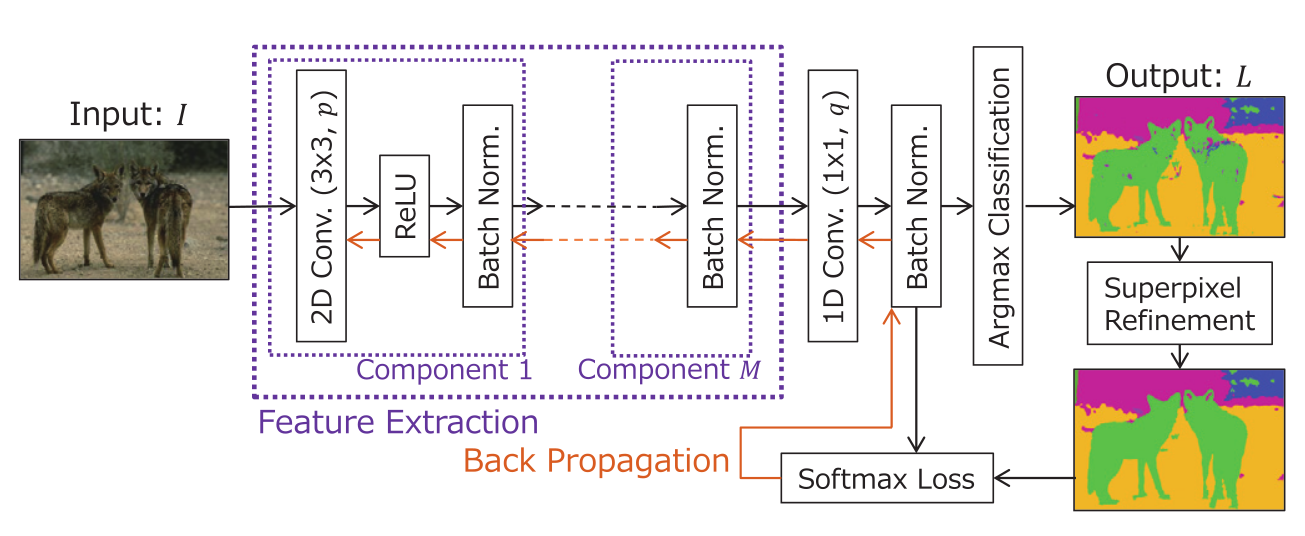
\includegraphics[height=20ex,keepaspectratio]{gfx/Kan18_01.png}
	\end{figure}
\end{frame}

\section{Methodik}

\begin{frame}{Funktionsweise}
\begin{minipage}{0.6\textwidth}
	\begin{itemize}
		\item \alert{Initialisierung} durch klassischen Clusteringalgorithmus
		\item \alert{Iterative Segmentierung} der Eingabe durch ein NN
		\begin{itemize}
			\item Vereinen der beiden Clusteringergebnisse
			\item Loss zwischen der Vereinigung und der NN-Ausgabe berechnen
			\item Das NN durch Backpropagation optimieren
		\end{itemize}
	\item \alert{Abbruchkriterium}
	\end{itemize}
\end{minipage}
\hfill
\begin{minipage}{0.38\textwidth}
	\begin{figure}[h!]
		\centering
		\begin{tikzpicture}[scale=.5,every node/.style={scale=0.5}]
		\draw  [draw, text width=7cm, align=center] (0,0) rectangle  node{Eingabebild} (7,-1);
		\path [->,>=stealth] (1.5,-1) edge (1.5,-1.5);
		\path [->,>=stealth] (5.5,-1) edge (5.5,-1.5);
		\draw  [draw, text width = 2.5cm, align=center] (0,-1.5) rectangle node{Neuronales Netzwerk mit Argmax Klassifizierung und Feature Extraction} (3,-5.5);
		\path [->,>=stealth] (1.5,-5.5) edge (1.5,-6);
		\draw  [draw, text width = 2.5cm, align=center] (4,-1.5) rectangle node{Clustering-algorithmus (bspw. SLIC)} (7,-5.5);
		\path [->,>=stealth] (5.5,-5.5) edge (5.5,-6);
		\draw  [dashed, text width = 3.5cm, align=center] (0,-6) rectangle node{Klasse jedes Pixels} (3.5,-6.5);
		\draw  [dashed, text width = 3.5cm, align=center] (3.5,-6) rectangle node{Pixelcluster} (7,-6.5);
		\draw (0,-6.5) -- (0,-8) -- (7,-8) -- (7,-6.5);
		\node [text width=6.5cm, align=center] at (3.5,-7.25) {Jedem Pixelcluster die in ihm häufigste Klasse zuweisen};
		\path [->,>=stealth] (3.5,-8) edge (3.5,-8.5);
		\draw  [draw, text width = 6.5cm, align=center] (0,-8.5) rectangle node{Loss berechnen} (7,-9.5);
		
		\path [-] (0,-5) edge (-0.5,-5);
		\path [-] (-0.5,-5) edge (-0.5,-9);
		\path [->,>=stealth] (-0.5,-9) edge (0,-9);
		
		\path [-] (3.5,-9.5) edge (3.5,-10);
		\path [-] (3.5,-10) edge (-1,-10);
		\path [-] (-1,-10) edge (-1,-2.75);
		\node [text width=6.5cm, align=center,rotate=90] at (-1.25,-6.5) {Optimiert durch Backpropagation};
		\path [->,>=stealth] (-1,-2.75) edge (0,-2.75);
		\end{tikzpicture}
		\caption{Übersicht über die Funktionsweise des Algorithmus}
	\end{figure}
\end{minipage}
\end{frame}
\begin{frame}{Initialisierung}
	\begin{minipage}{0.65\textwidth}
		\begin{itemize}
			\item Im Ansatz nach Kanezaki wird SLIC genutzt
			\begin{itemize}
				\item Nur Farb- und Positionsbasiert
				\item Schlechte Resultate bei S/W-Marsaufnahmen
				\item NN würde lernen, anhand der Helligkeit zu segmentieren
			\end{itemize}
			\item Stattdessen texturbasiertes Clustering
			\begin{itemize}
				\item NN erlernt, nach den Texturen zu segmentieren
				\item Besser, da Oberflächenmerkmale meist anhand ihrer Texturen unterschieden werden
			\end{itemize}
		\end{itemize}
	\end{minipage}
	\hfill
	\begin{minipage}{0.20\textwidth}
		\begin{figure}[h!]
			\begin{subfigure}{\textwidth}
				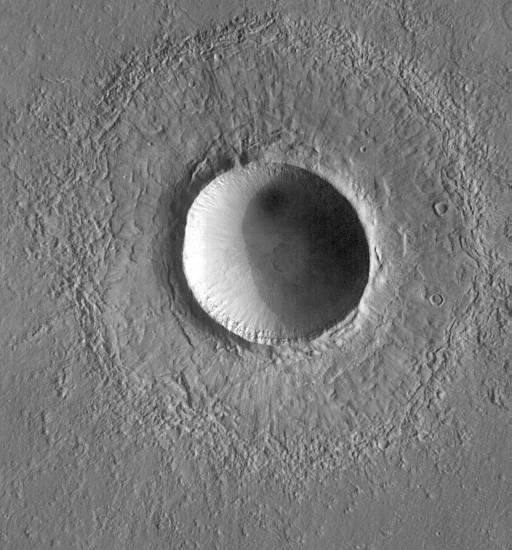
\includegraphics[width=\textwidth,keepaspectratio]{gfx/Gre13_01.jpg}
			\end{subfigure}
			\begin{subfigure}{\textwidth}
				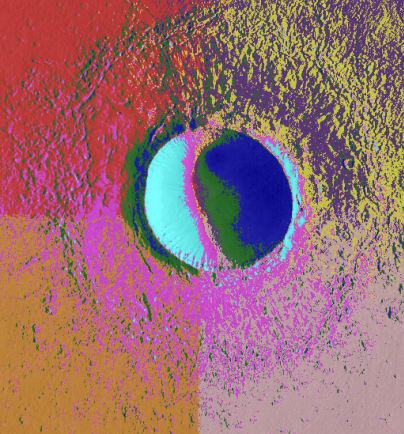
\includegraphics[width=\textwidth,keepaspectratio]{gfx/Gre13_01.jpg_slic.png}
			\end{subfigure}
			\begin{subfigure}{\textwidth}
				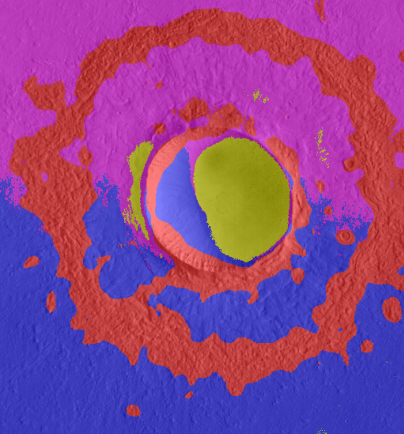
\includegraphics[width=\textwidth,keepaspectratio]{gfx/Gre13_01.jpg_tsugf.png}
			\end{subfigure}
		\end{figure}
	\end{minipage}
\end{frame}

\begin{frame}{Texturbasiertes Clustering}
Vergleich von Textur in benachbarten Bereichen:
	\begin{itemize}
		\item Anwendung von unterschiedlichen Gabor-Filtern:
		\begin{figure}
			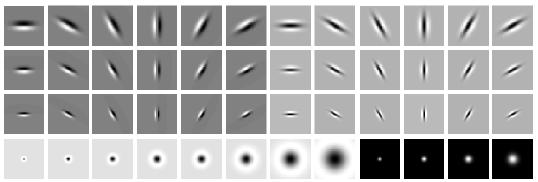
\includegraphics[width=.5\textwidth,keepaspectratio]{gfx/vis_01.jpg}
		\end{figure}
		\item Optimierung der Filter-Ergebnisse (Weichnzeichnen)
		\item Erweiterung des Datenwürfels um Positions- und Farb-Merkmale\footnote{Anpassbare Gewichtungen}
		\item Anschließend eigentliches Clustering über k-Means
\end{itemize}
\end{frame}

\begin{frame}{Texturbasiertes Clustering - Abbildungen}
	\begin{figure}
		\begin{subfigure}[t]{.3\textwidth}
			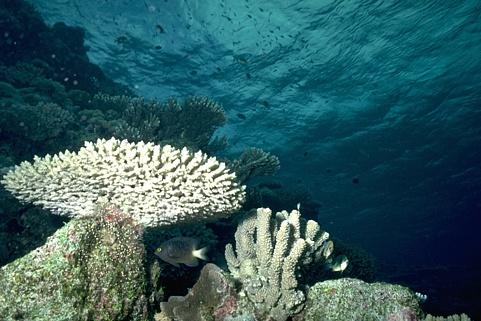
\includegraphics[width=\textwidth,keepaspectratio]{gfx/101027.jpg}
			\caption{Eingabedatei, aus \cite{bsd500}}
		\end{subfigure}
		\hfill
			\begin{subfigure}[t]{.3\textwidth}
			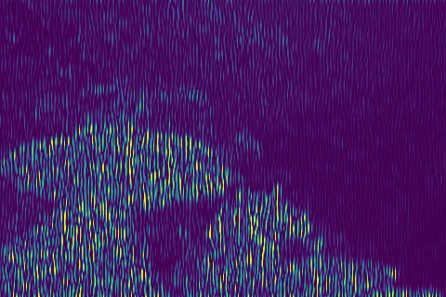
\includegraphics[width=\textwidth,keepaspectratio]{gfx/101027.jpg_0.png}
			\caption{Resultat der Anwendung \emph{eines} Gabor-Filters}
		\end{subfigure}
		\hfill
		\begin{subfigure}[t]{.3\textwidth}
			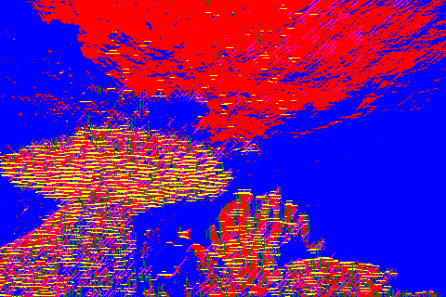
\includegraphics[width=\textwidth,keepaspectratio]{gfx/101027.jpg_raw.png}
			\caption{Clusteringergebnis ohne Optimierungen}
		\end{subfigure}\\
		\begin{subfigure}[t]{.3\textwidth}
			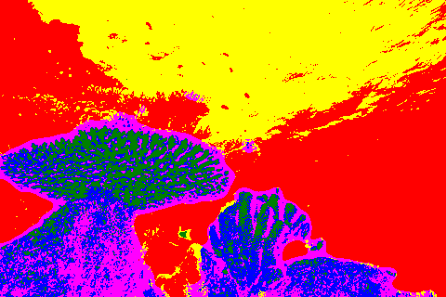
\includegraphics[width=\textwidth,keepaspectratio]{gfx/101027.jpg_blur.png}
			\caption{Clusteringergebnis mit Weichzeichnung}
		\end{subfigure}
		\hfill
		\begin{subfigure}[t]{.3\textwidth}
			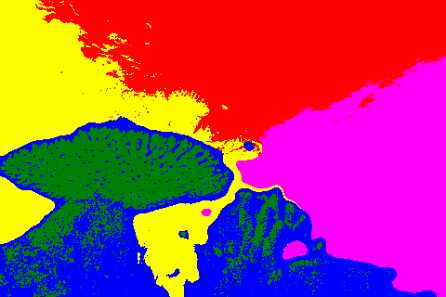
\includegraphics[width=\textwidth,keepaspectratio]{gfx/101027.jpg_blur_norm_spatial.png}
			\caption{Clusteringergebnis mit Weichzeichnung und Positionswerten}
		\end{subfigure}
		\hfill
		\begin{subfigure}[t]{.3\textwidth}
			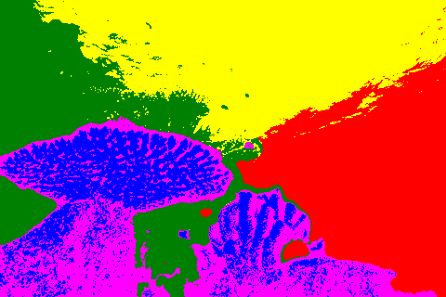
\includegraphics[width=\textwidth,keepaspectratio]{gfx/101027.jpg_blur_norm_spatial_color.png}
			\caption{Clusteringergebnis mit Weichzeichnung, Normalisierung, Farbwerten und Positionswerten}
		\end{subfigure}
		\caption{Texturbasiertes Clustering}
	\end{figure}
\end{frame}

\begin{frame}{Iterative Segmentierung}
	\begin{itemize}
		\item Iteratives durchlaufen eines NN schichtweise bestehend aus:
		\begin{itemize}
			\item Convolutional Layer
			\item Batch Normalization
			\item ReLU $\rightarrow$ Von den getesteten Aktivierungsfunktionen am besten geeignet
		\end{itemize}
		\item Keine Verbesserungen wurden erreicht durch:
		\begin{itemize}
			\item Pooling Layer
			\item Fully Connected Layer
		\end{itemize}
		\medskip
		\item Anschließend wird das NN-Ergebnis mit dem des klassischen Clusterings optimiert
		\item Loss zwischen NN-Ergebnis unnd klassischem Ergebnis als Qualitätsmaß für folgende Backpropagation
	\end{itemize}
\end{frame}

\begin{frame}{Abbruchkriterium}
	\begin{itemize}
		\item Ursprünglicher Algorithmus nach Kanezaki:
		\begin{itemize}
			\item Anzahl der Segmente
		\end{itemize}
		\item Alternativen:
		\begin{itemize}
			\item Wert der Verlustfunktion
			\item Median der relativen Änderung in den letzten $n$ Epochen
			\item Ableitung einer Annäherung an die Verlustfunktion
		\end{itemize}
	\end{itemize}

\end{frame}

\begin{frame}{Abbruchkriterium - Abbildungen}
	\vspace*{-0.8cm}
	\begin{figure}[h!]
		\footnotesize
		\hspace*{-0.8cm}
		\begin{tikzpicture}
		\begin{groupplot}[
		group style={
			group size=2 by 2,
			vertical sep=1.25cm,
			horizontal sep=1.8cm
		},
		width=0.55\textwidth,
		height=4.5cm]
		\nextgroupplot[major grid style={line width=.1pt, draw=gray!30},
		minor grid style={line width=.1pt, draw=gray!10},
		minor tick num=3,
		grid=both,
		xmin=0,
		xmax=300,
		ymin=0,
		ymax=30,
		xlabel style={text width=3cm,align=center},
		xlabel=Epoche,
		ylabel=Segmente]
		\addplot +[mark=none,blue,smooth] table [x=Step, y=Value, col sep=comma] {data/stoppingcriteria/run-1585332321.2379851_p03_01.png-tag-labels_.csv};
		\addplot +[mark=none,red,smooth] table [x=Step, y=Value, col sep=comma] {data/stoppingcriteria/run-1585332321.2379851_p03_02.png-tag-labels_.csv};
		\addplot +[mark=none,green,smooth] table [x=Step, y=Value, col sep=comma] {data/stoppingcriteria/run-1585332321.2379851_p03_03.png-tag-labels_.csv};
		\addplot +[mark=none,black,smooth] table [x=Step, y=Value, col sep=comma] {data/stoppingcriteria/run-1585332321.2379851_p03_04.png-tag-labels_.csv};
		
		\nextgroupplot[major grid style={line width=.1pt, draw=gray!30},
		minor grid style={line width=.1pt, draw=gray!10},
		minor tick num=3,
		grid=both,
		xmin=0,
		xmax=300,
		ymin=0,
		ymax=2.5,
		xlabel style={text width=6cm,align=center},
		xlabel=Epoche,
		ylabel=Loss]
		\addplot +[mark=none,blue,smooth] table [x=Step, y=Value, col sep=comma] {data/stoppingcriteria/run-1585332321.2379851_p03_01.png-tag-loss_loss.csv};
		\addplot +[mark=none,red,smooth] table [x=Step, y=Value, col sep=comma] {data/stoppingcriteria/run-1585332321.2379851_p03_02.png-tag-loss_loss.csv};
		\addplot +[mark=none,green,smooth] table [x=Step, y=Value, col sep=comma] {data/stoppingcriteria/run-1585332321.2379851_p03_03.png-tag-loss_loss.csv};
		\addplot +[mark=none,black,smooth] table [x=Step, y=Value, col sep=comma] {data/stoppingcriteria/run-1585332321.2379851_p03_04.png-tag-loss_loss.csv};
		\nextgroupplot[major grid style={line width=.1pt, draw=gray!30},
		minor grid style={line width=.1pt, draw=gray!10},
		minor tick num=3,
		grid=both,
		xmin=0,
		xmax=300,
		ymin=-0.03,
		ymax=0.01,
		xlabel style={text width=5cm,align=center},
		xlabel=Epoche,
		ylabel=Median der Verlustfunktionin den letzten 20 Epochen,
		ylabel style={text width=4cm,align=center},
		legend style={at={(0.02,0.98)}, anchor=north west}]
		\addplot +[mark=none,blue,smooth] table [x=Step, y=Value, col sep=comma] {data/stoppingcriteria/run-1585332321.2379851_p03_01.png-tag-loss_delta_over_20.csv};
		\addplot +[mark=none,red,smooth] table [x=Step, y=Value, col sep=comma] {data/stoppingcriteria/run-1585332321.2379851_p03_02.png-tag-loss_delta_over_20.csv};
		\addplot +[mark=none,green,smooth] table [x=Step, y=Value, col sep=comma] {data/stoppingcriteria/run-1585332321.2379851_p03_03.png-tag-loss_delta_over_20.csv};
		\addplot +[mark=none,black,smooth] table [x=Step, y=Value, col sep=comma] {data/stoppingcriteria/run-1585332321.2379851_p03_04.png-tag-loss_delta_over_20.csv};
		
		\nextgroupplot[major grid style={line width=.1pt, draw=gray!30},
		minor grid style={line width=.1pt, draw=gray!10},
		minor tick num=3,
		grid=both,
		xmin=0,
		xmax=300,
		ymin=-0.03,
		ymax=0.01,
		xlabel=Epoche,
		ylabel=Approximierter Gradient der Verlustfunktion,
		ylabel style={text width=4cm,align=center},
		legend style={at={(0.02,0.98)}, anchor=north west}]
		\addplot +[mark=none,blue,smooth] table [x=Step, y=Value, col sep=comma] {data/stoppingcriteria/run-1585332321.2379851_p03_01.png-tag-approx_deriv.csv};
		\addplot +[mark=none,red,smooth] table [x=Step, y=Value, col sep=comma] {data/stoppingcriteria/run-1585332321.2379851_p03_02.png-tag-approx_deriv.csv};
		\addplot +[mark=none,green,smooth] table [x=Step, y=Value, col sep=comma] {data/stoppingcriteria/run-1585332321.2379851_p03_03.png-tag-approx_deriv.csv};
		\addplot +[mark=none,black,smooth] table [x=Step, y=Value, col sep=comma] {data/stoppingcriteria/run-1585332321.2379851_p03_04.png-tag-approx_deriv.csv};
		
		\end{groupplot}
		\end{tikzpicture}
	\end{figure}
\end{frame}

\begin{frame}{Zu Optimierende Parameter}
\begin{itemize}
	\item Auswahl der Filterbank
	\item Größe der Filter
	\item Gewichtung von Farb-/Positions-Werten
	\item Anzahl der Cluster
	\item Abbruchkriterium
	\item Aktivierungsfunktion
	\item Zusätzliche Schichten wie Pooling oder Fully Connected Layers
	\item Anzahl, Größe, Stride der Konvolutionsschichten
\end{itemize}
\end{frame}

\section{Resultate}

\begin{frame}[allowframebreaks]{Resultate - Domänenspezifisch}
	\begin{figure}[h!]
		\begin{subfigure}{0.38\textwidth}
			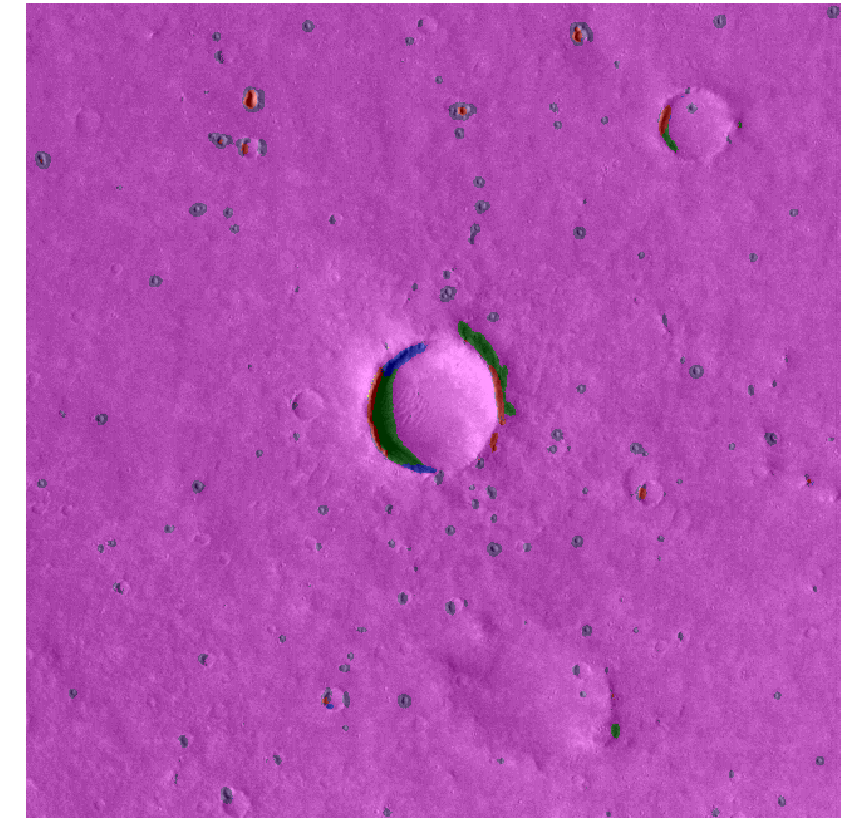
\includegraphics[width=\linewidth,keepaspectratio]{gfx/p03_01.png_3.png}
		\end{subfigure}
		\begin{subfigure}{0.38\textwidth}
			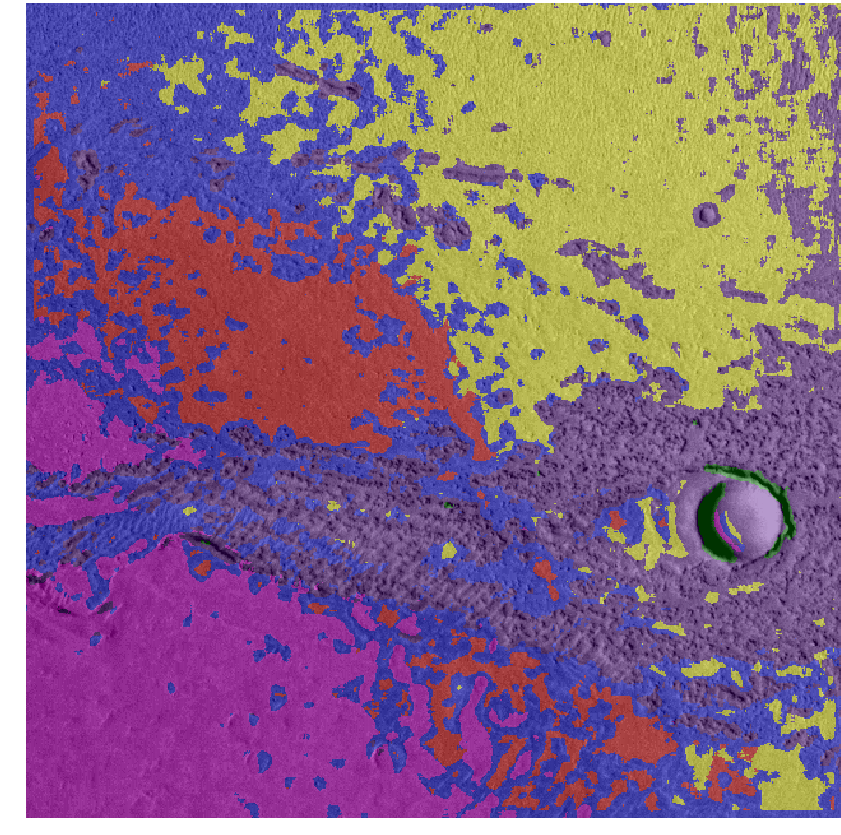
\includegraphics[width=\linewidth,keepaspectratio]{gfx/p03_02.png_3.png}
		\end{subfigure}
		\\
		\begin{subfigure}{0.38\textwidth}
			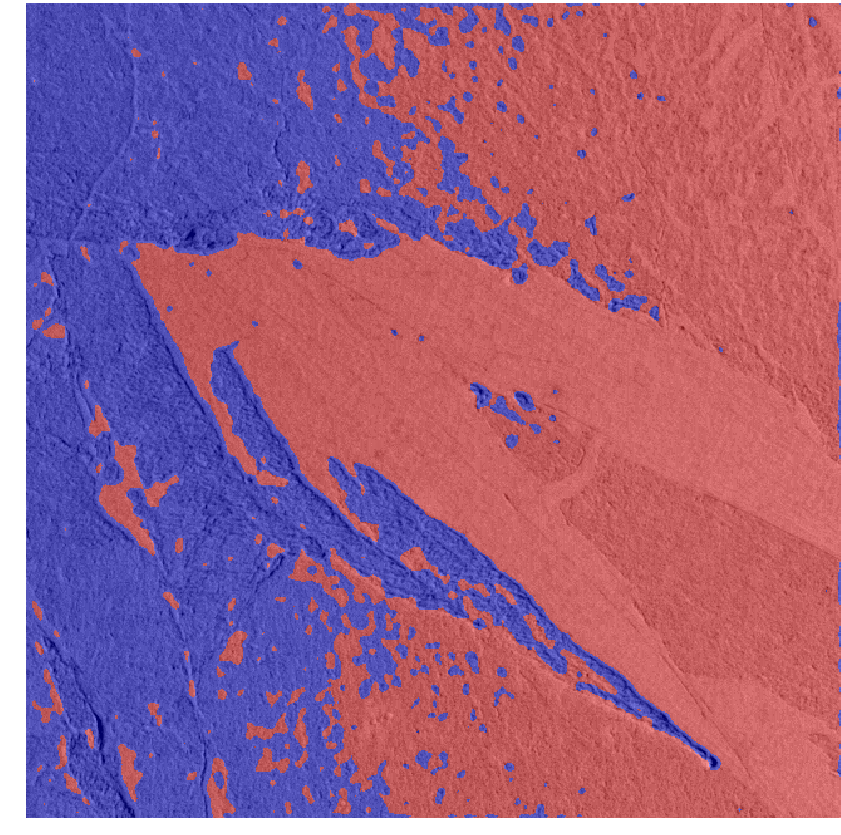
\includegraphics[width=\linewidth,keepaspectratio]{gfx/p03_03.png_3.png}
		\end{subfigure}
		\begin{subfigure}{0.38\textwidth}
			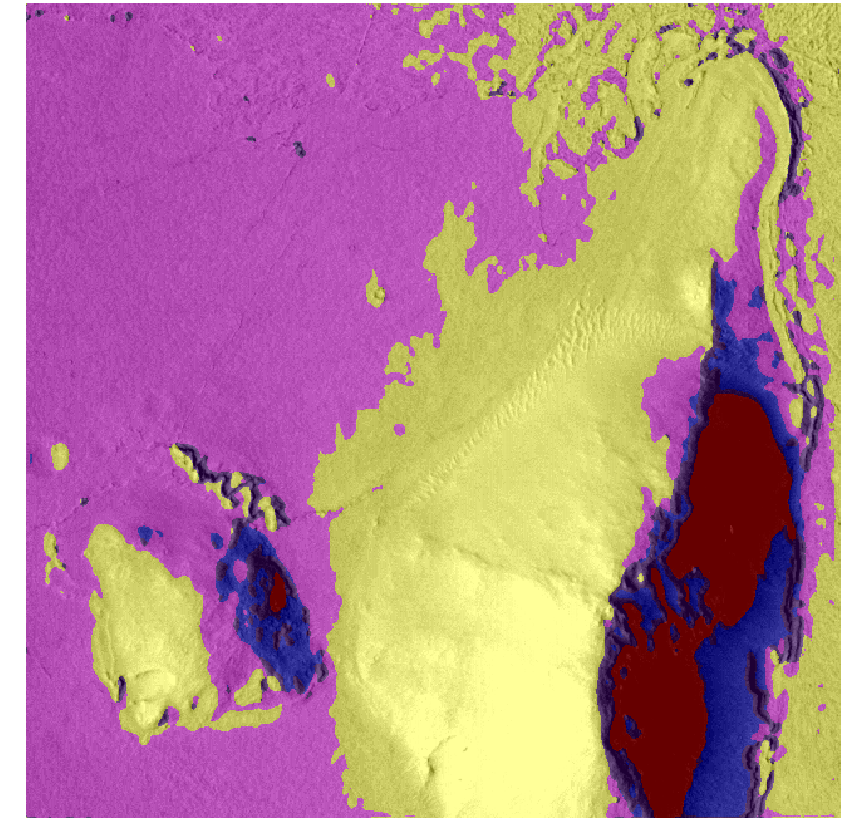
\includegraphics[width=\linewidth,keepaspectratio]{gfx/p03_04.png_3.png}
		\end{subfigure}
	\end{figure}
	\newpage
	Ausgabe musste menschlich annotiert werden, um auf vorhandenen Datensätzen evaluiert werden zu können.\\\vspace{10pt}
	\begin{minipage}{0.58\textwidth}
		\footnotesize
		\begin{table}[h!]
			\begin{tabularx}{\textwidth}{p{0.49\textwidth} >{\centering\arraybackslash}p{0.49\textwidth}}
				\toprule
				\textbf{Algorithmus} & \textbf{$F_1$-Score\footnotemark} \\
				\midrule
				Urbach 09 \cite{urbach_stepinski_2009} & $0,7243$ \\
				Bandeira 10 \cite{bandeira_10} & $0,8359$ \\
				Ding 11 \cite{ding_11} & $0,8550$ \\
				Cohen 16 \cite{cohen_16} \footnotemark[3] & $0,8929$ \\
				\textbf{Unüberwachtes tiefes Clustering} & $0,6374$\\
				\bottomrule
			\end{tabularx}
			%\caption{Vergleich der durchschnittlichen $F_1$-Scores unterschiedlicher Algorithmen zur Kratererkennung. Die Daten wurden aus \cite{cohen_16} übernommen.}
		\end{table}
	\end{minipage}
	\hfill
	\begin{minipage}{0.38\textwidth}
		\begin{figure}[h!]
			\begin{subfigure}[t]{0.31\textwidth}
				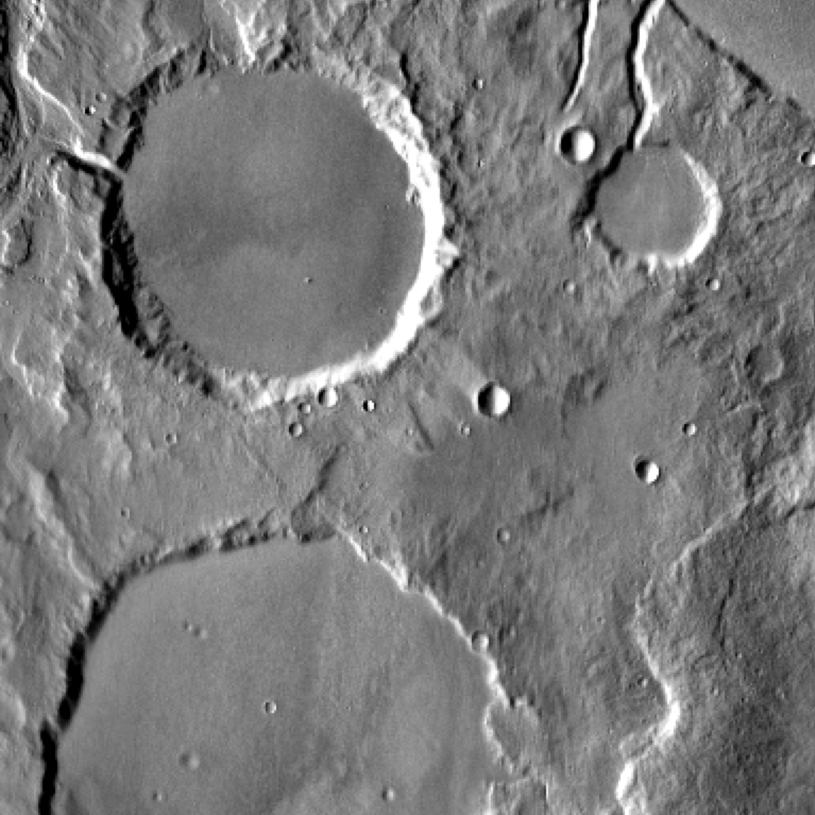
\includegraphics[width=\linewidth,keepaspectratio]{gfx/rob_in/thm_dir_N-30_210.png_sourcetile_60.png}
			\end{subfigure}
			\begin{subfigure}[t]{0.31\textwidth}
				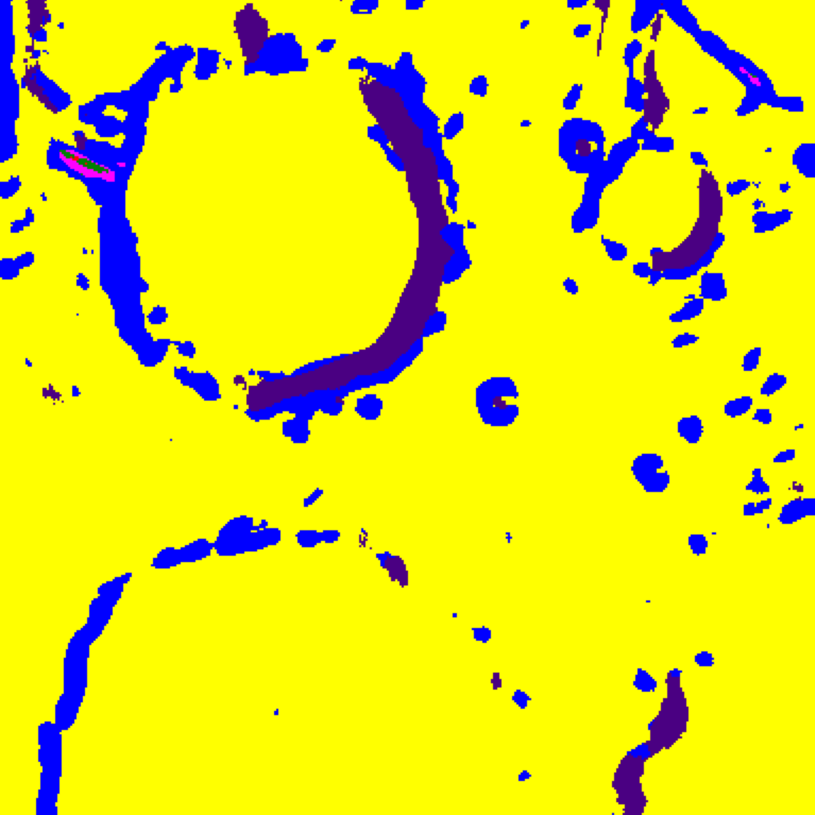
\includegraphics[width=\linewidth,keepaspectratio]{gfx/rob_res/thm_dir_N-30_210.png_tile_60.png}
			\end{subfigure}
			\begin{subfigure}[t]{0.31\textwidth}
			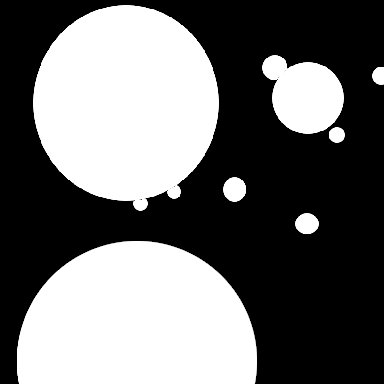
\includegraphics[width=\linewidth,keepaspectratio]{gfx/rob_hum/thm_dir_N-30_210.png_tile_60.png}
			\end{subfigure}\\
			\begin{subfigure}[t]{0.31\textwidth}
				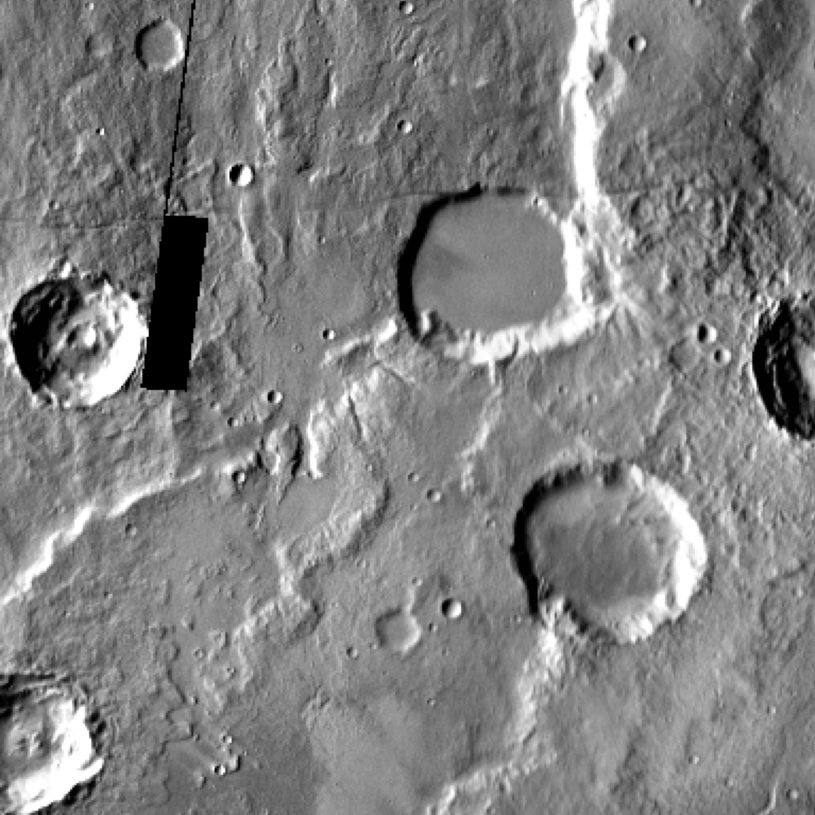
\includegraphics[width=\linewidth,keepaspectratio]{gfx/rob_in/thm_dir_N-30_210.png_sourcetile_100.png}
			\end{subfigure}
			\begin{subfigure}[t]{0.31\textwidth}
				
\includegraphics[width=\linewidth,keepaspectratio]{gfx/rob_res/thm_dir_N-30_210.png_tile_100.png}
			\end{subfigure}
			\begin{subfigure}[t]{0.31\textwidth}
				
\includegraphics[width=\linewidth,keepaspectratio]{gfx/rob_hum/thm_dir_N-30_210.png_tile_100.png}
			\end{subfigure}\\
			\begin{subfigure}[t]{0.31\textwidth}
				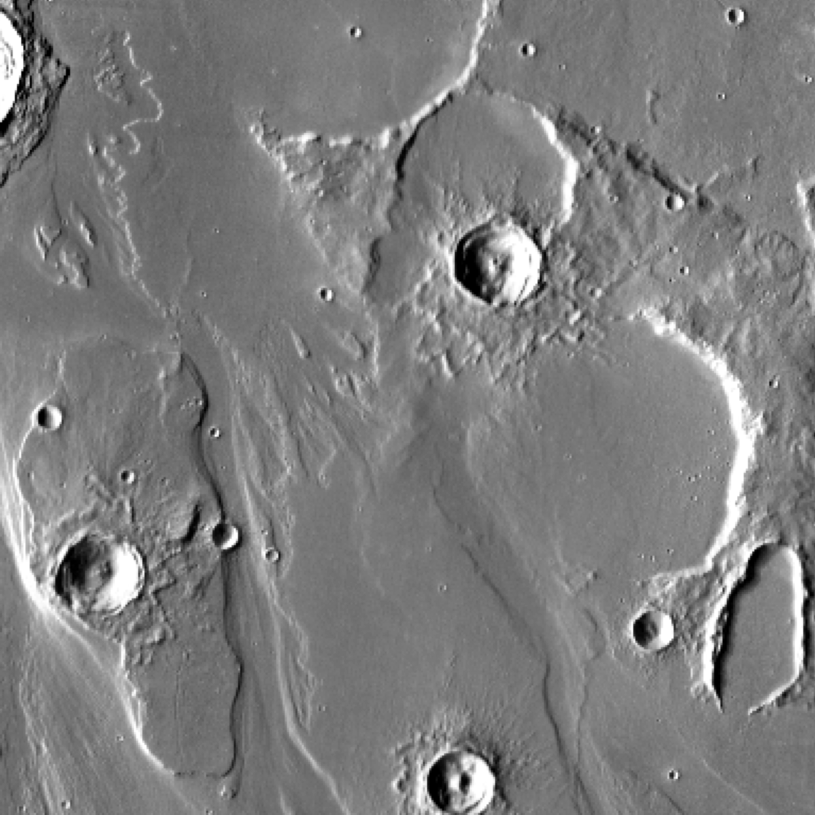
\includegraphics[width=\linewidth,keepaspectratio]{gfx/rob_in/thm_dir_N-30_210.png_sourcetile_160.png}
				\caption{Eingabedatei}
			\end{subfigure}
			\begin{subfigure}[t]{0.31\textwidth}
				
\includegraphics[width=\linewidth,keepaspectratio]{gfx/rob_res/thm_dir_N-30_210.png_tile_160.png}
				\caption{Ausgabe}
			\end{subfigure}
			\begin{subfigure}[t]{0.31\textwidth}
				
\includegraphics[width=\linewidth,keepaspectratio]{gfx/rob_hum/thm_dir_N-30_210.png_tile_160.png}
				\caption{Menschlich annotierte Ausgabe}
			\end{subfigure}
		\end{figure}
	\end{minipage}
	\footnotetext{Daten aus \cite{cohen_16}}
	\footnotetext[3]{Überwacht}
\end{frame}

\begin{frame}{Resultate - Allgemein}
	\begin{minipage}{0.6\textwidth}
		\footnotesize
		\begin{table}[h!]
			\begin{tabularx}{\textwidth}{p{0.40\textwidth} >{\centering} p{0.24\textwidth} >{\centering\arraybackslash} p{0.24\textwidth}}
				\toprule
				\textbf{Methode} & \textbf{PRI\footnotemark[4]} & \textbf{VoI\footnotemark[4]} \\
				\midrule
				Mensch \cite{bsd500} & $0,88$ & $1,17$ \\
				\midrule
				gPb-pwt-ucm \cite{arbelaez_10} & $0,83$ & $1,69$ \\
				Mean Shift \cite{comaniciu_02} & $0,79$ & $1,85$ \\
				Felz-Hutt \cite{felzenszwalb_04} & $0,80$ & $2,21$ \\
				Canny-owt-ucm \cite{arbelaez_10} & $0,79$ & $2,19$ \\
				NCuts \cite{cour_05} & $0,78$ & $2,23$ \\
				Quad-Tree & $0,73$ & $2,46$ \\
				\textbf{Unüberwachtes tiefes Clustering} & $0,73$ & $2,88$ \\
				\bottomrule
			\end{tabularx}
		\end{table}
	\end{minipage}
	\hfill
	\begin{minipage}{0.28\textwidth}
		\begin{figure}[h!]
			\begin{subfigure}{\textwidth}
				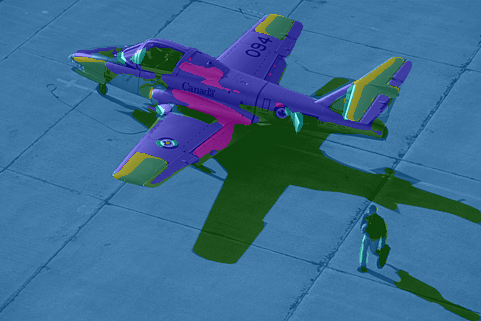
\includegraphics[width=\linewidth,keepaspectratio]{gfx/37073.jpg_seg.png}
			\end{subfigure}\\
			\begin{subfigure}{\textwidth}
				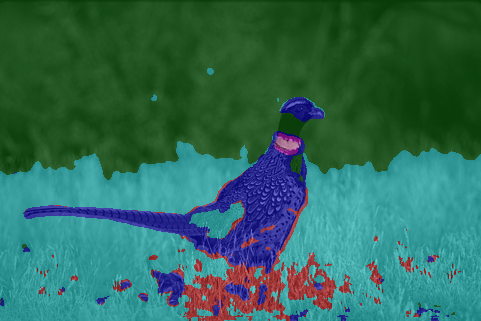
\includegraphics[width=\linewidth,keepaspectratio]{gfx/43074.jpg_seg.png}
			\end{subfigure}\\
			\begin{subfigure}{\textwidth}
				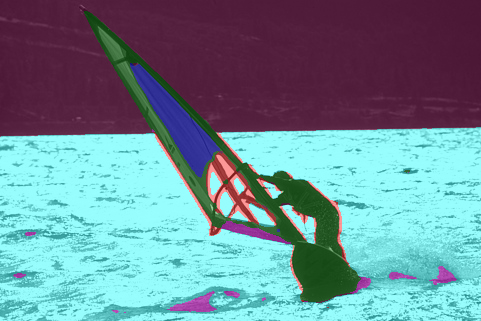
\includegraphics[width=\linewidth,keepaspectratio]{gfx/62096.jpg_seg.png}
			\end{subfigure}\\
			%\begin{subfigure}{0.3\textwidth}
			%	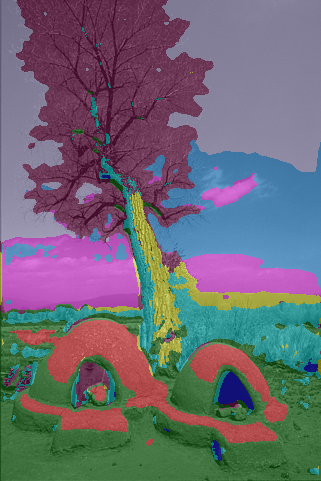
\includegraphics[width=\linewidth,keepaspectratio]{gfx/54082.jpg_seg.png}
			%\end{subfigure}
		\end{figure}
	\end{minipage}
	\footnotetext[4]{Daten aus \cite{arbelaez_10}}
\end{frame}

\section{Abschluss}

\begin{frame}{Aussicht}
	
\end{frame}

\begin{frame}{Fazit}
	
\end{frame}

\begin{frame}[allowframebreaks]{Referenzen}
	\setbeamertemplate{bibliography item}[text]
	\bibliographystyle{alpha}
	\bibliography{literatur}
\end{frame}
\end{document}